\begin{frame}[allowframebreaks]{Predicting One View from Another}

    \textbf{Learn to translate between modalities or augmentations}
    \begin{itemize}
        \item The core idea is to train a model that can predict or reconstruct one view of the data given another.
        \item Views can be different modalities (e.g., infrared vs. RGB), or different augmentations (e.g., color vs. grayscale, rotated images, etc.).
        \item This approach encourages the model to learn shared representations that capture the underlying semantics of the data, rather than superficial features.
    \end{itemize}

    \framebreak

    \begin{figure}
        \flushleft
        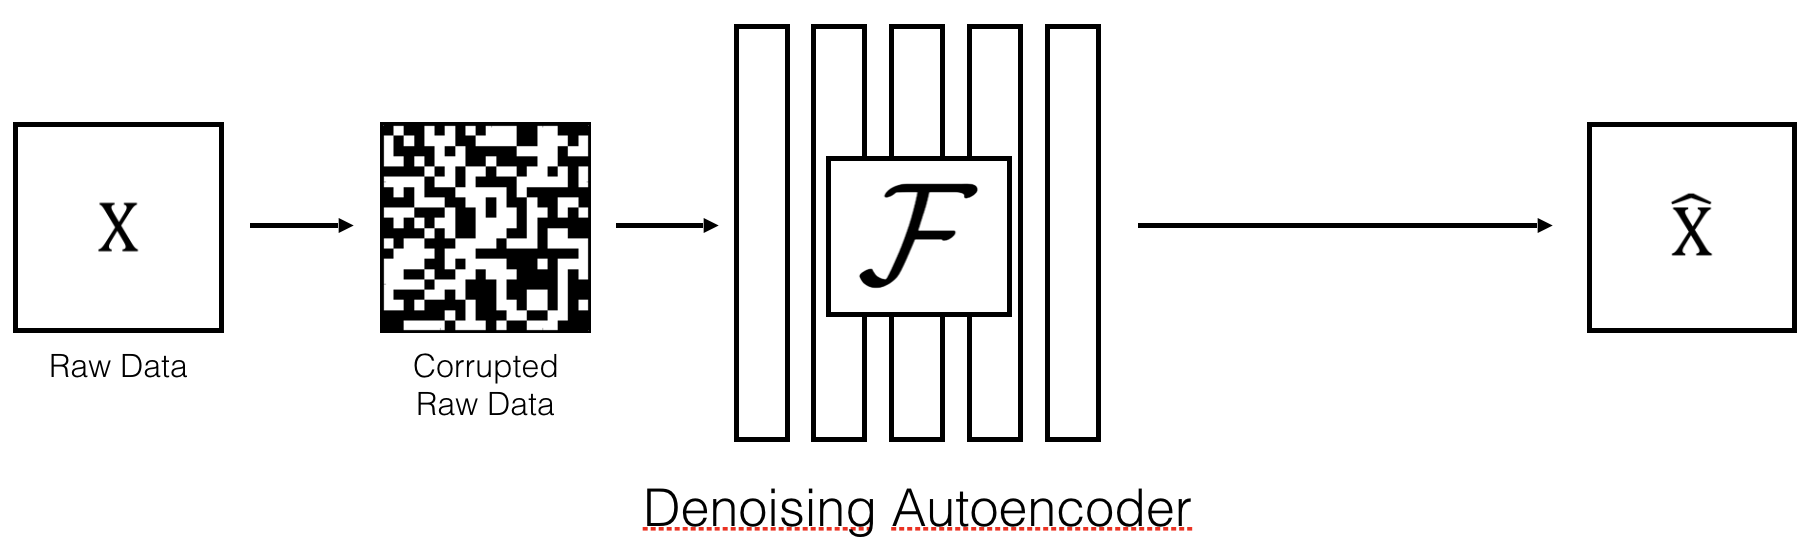
\includegraphics[width=1\linewidth,height=\textheight,keepaspectratio]{images/ssl/slide_24_1_img.png}
        Slide: Richard Zhang (2019). Predicting One View from Another.
    \end{figure}

    \framebreak

    \begin{figure}
        \flushleft
        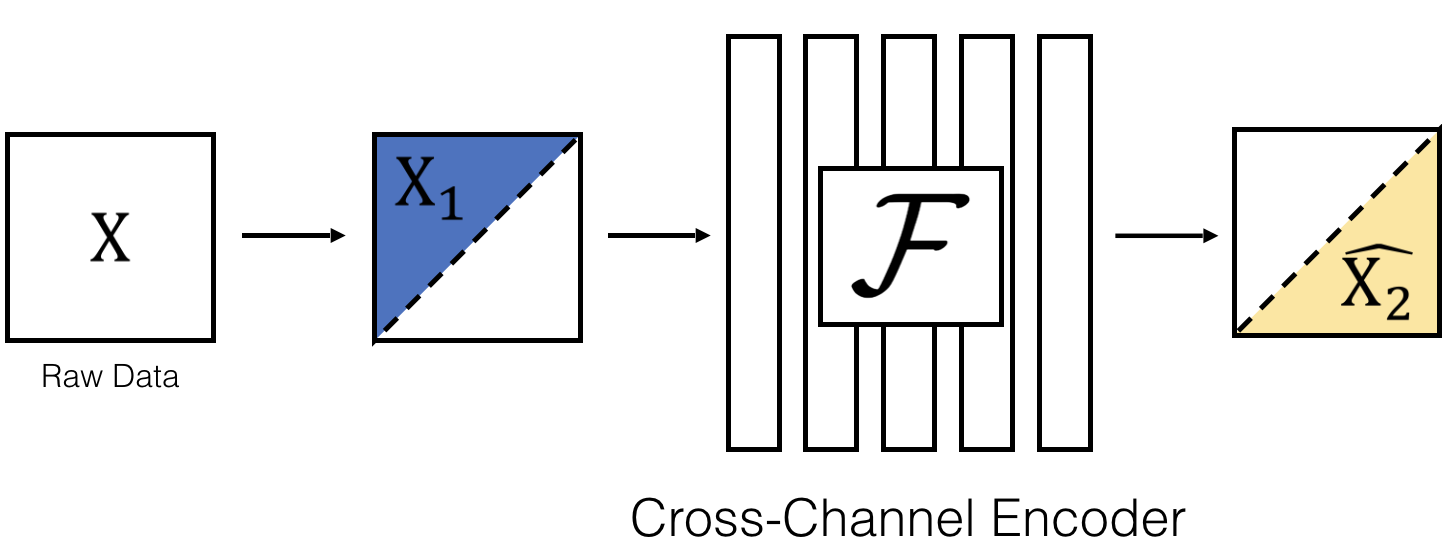
\includegraphics[width=1\linewidth,height=\textheight,keepaspectratio]{images/ssl/slide_25_1_img.png}
        Slide: Richard Zhang (2019). Predicting One View from Another.
    \end{figure}

    \framebreak

    \textbf{Example: Learn mapping from infrared to RGB imagery}
    \begin{itemize}
        \item In remote sensing, images are often captured in both infrared and RGB channels.
        \item A model can be trained to predict the RGB image given the infrared image, or vice versa.
        \item This task forces the model to understand the relationship between the two modalities, which can improve its generalization and robustness.
        \item Such cross-modal prediction is useful for applications where one modality may be missing or corrupted.
    \end{itemize}

    \framebreak

    \begin{figure}
        \flushleft
        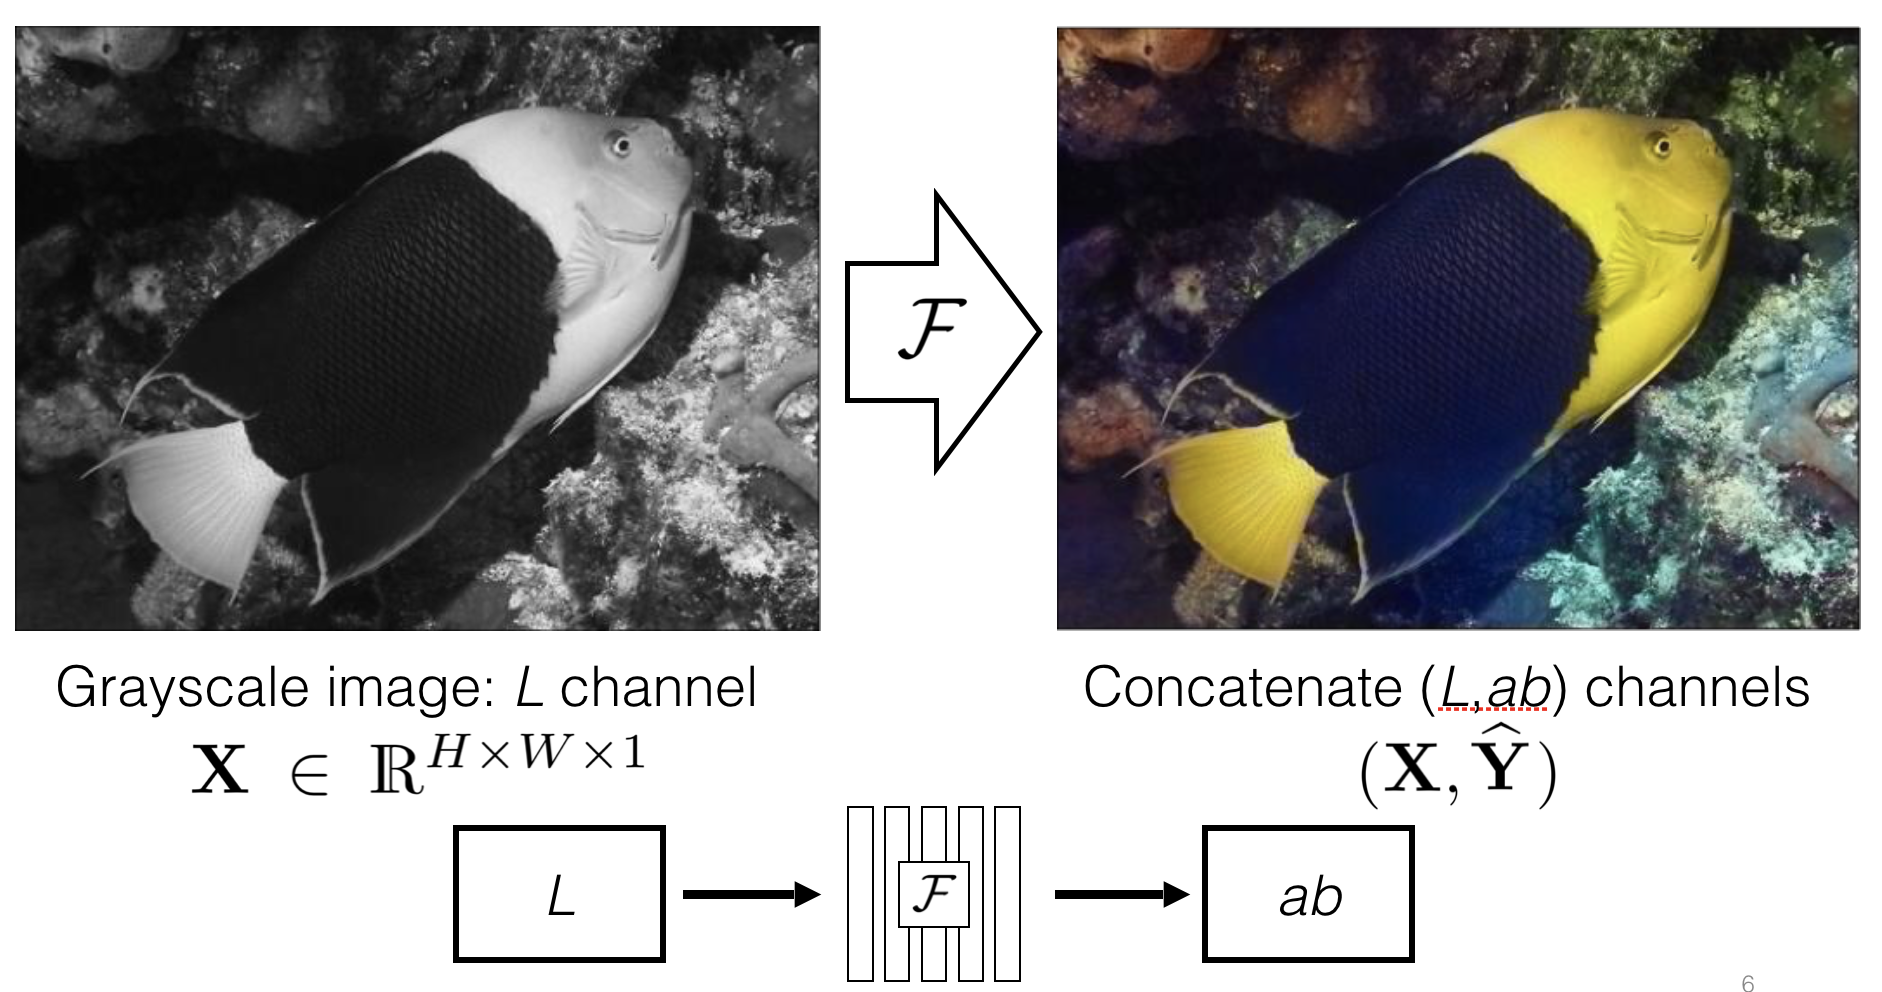
\includegraphics[width=1\linewidth,height=\textheight,keepaspectratio]{images/ssl/slide_26_1_img.png}
        Slide: Richard Zhang (2019). Predicting One View from Another.
    \end{figure}

    \framebreak

    \begin{figure}
        \flushleft
        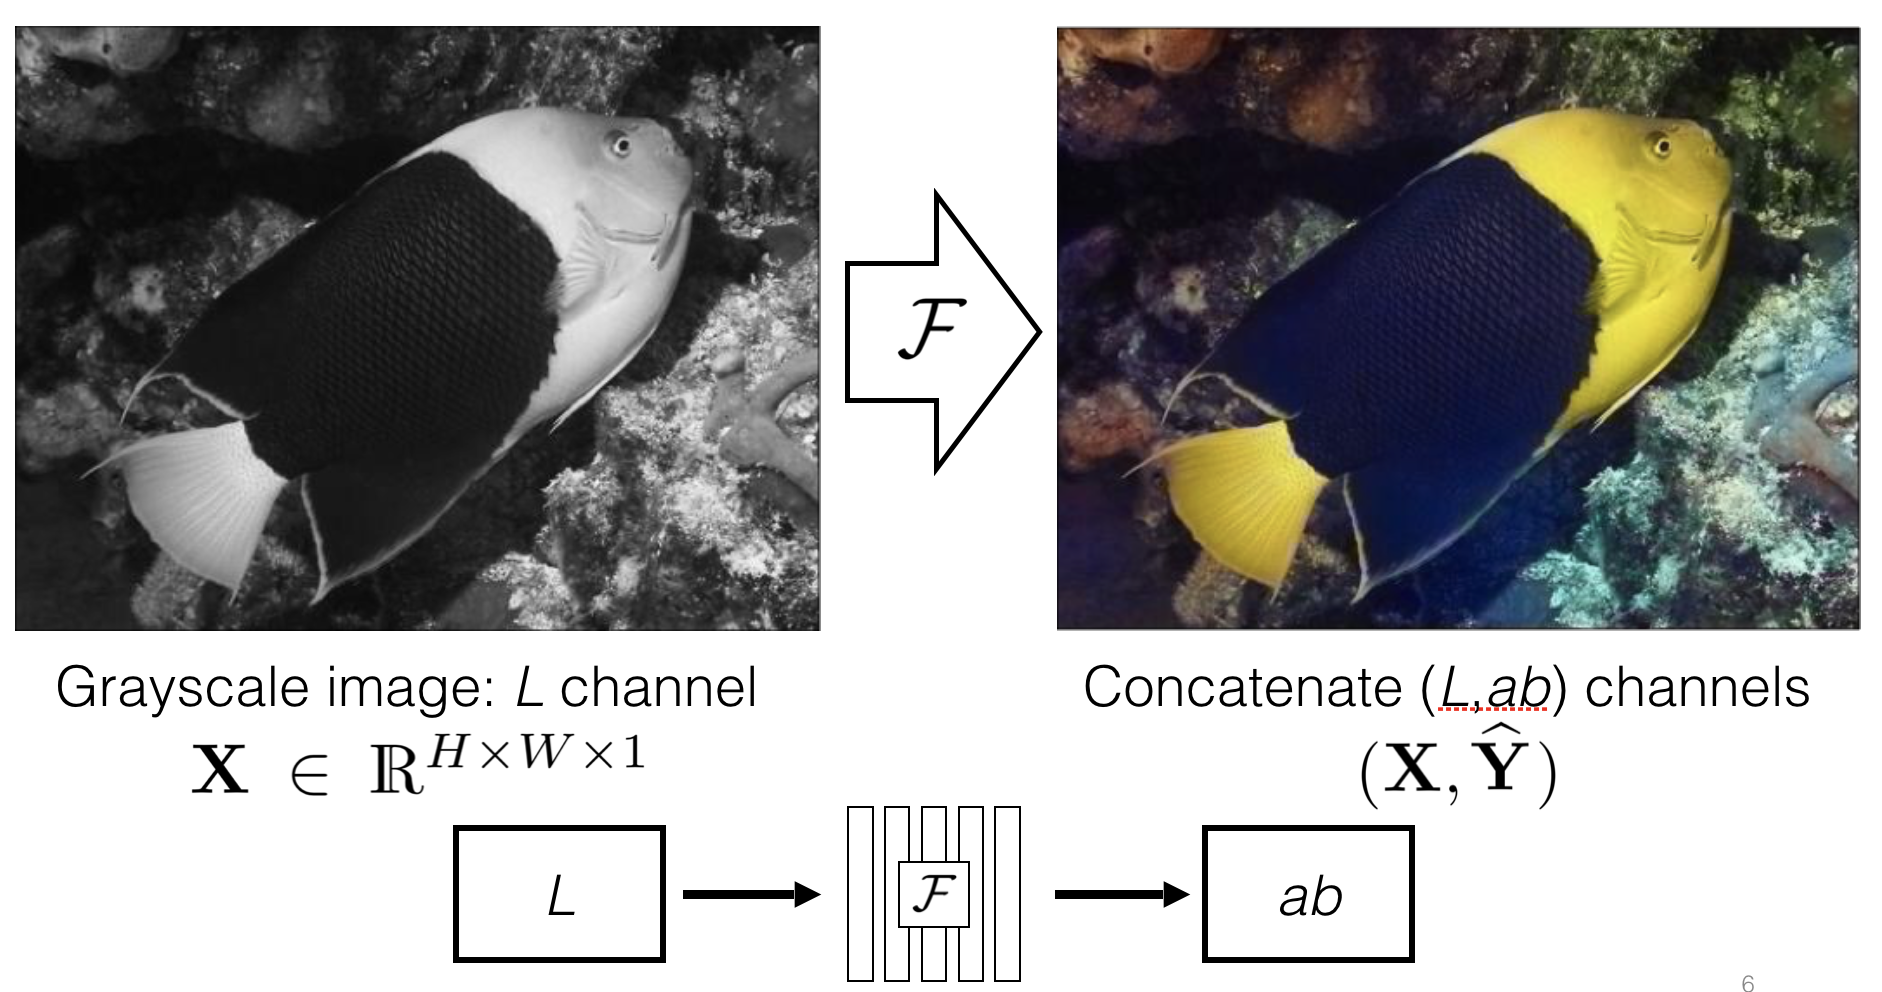
\includegraphics[width=1\linewidth,height=\textheight,keepaspectratio]{images/ssl/slide_27_1_img.png}
        Slide: Richard Zhang (2019). Predicting One View from Another.
    \end{figure}

    \framebreak

    \begin{figure}
        \flushleft
        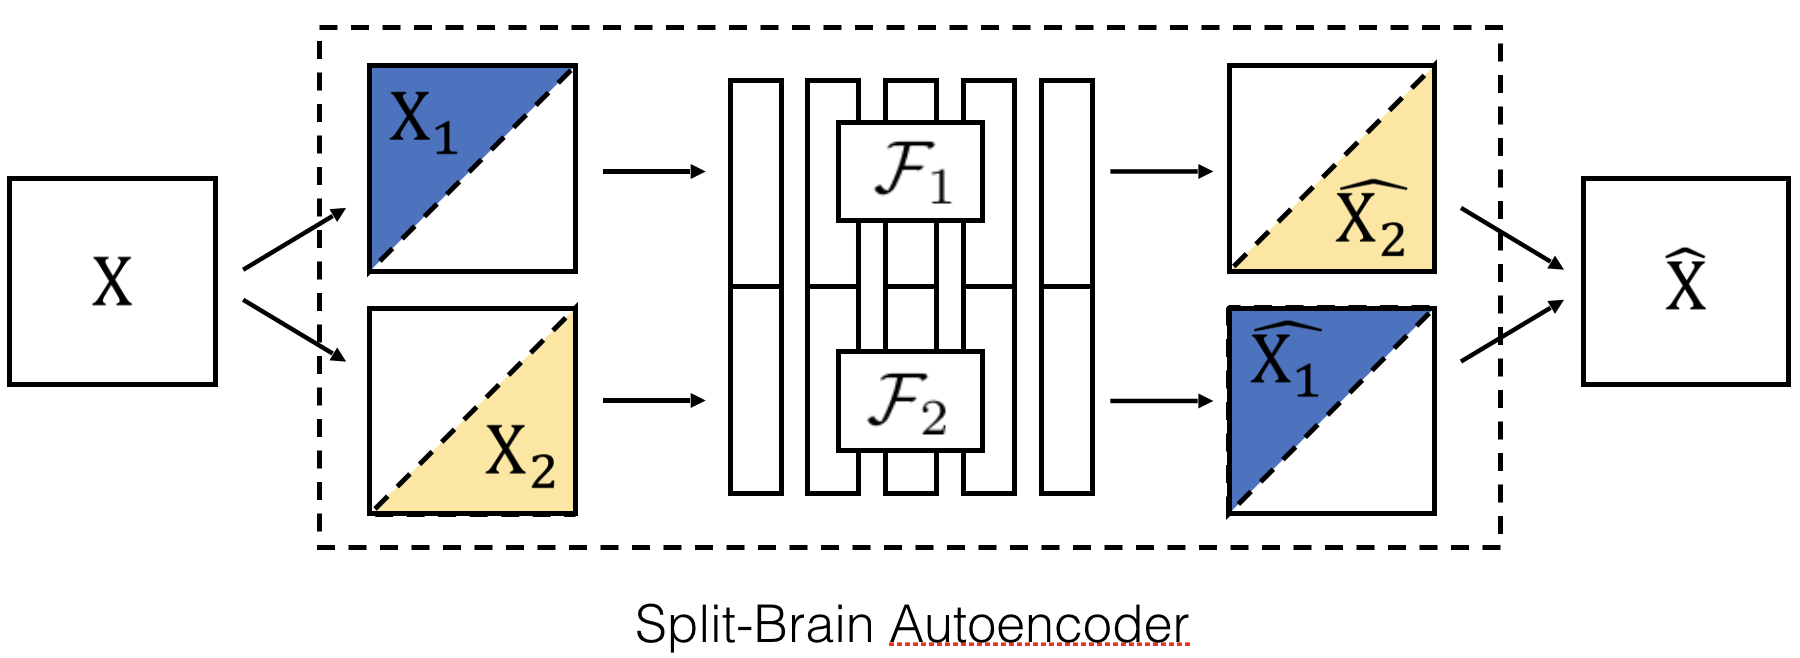
\includegraphics[width=1\linewidth,height=\textheight,keepaspectratio]{images/ssl/slide_28_1_img.png}
        Slide: Richard Zhang (2019). Predicting One View from Another.
    \end{figure}

    \framebreak
    
    \begin{itemize} 
        \item \textbf{Applications and Benefits}
        \begin{itemize}
            \item \textbf{Data augmentation}: By learning to predict one augmentation from another, models become more invariant to transformations.
            \item \textbf{Multi-modal learning}: Enables leveraging complementary information from different data sources.
            \item \textbf{Self-supervised learning}: No need for manual labels, as the prediction task itself provides the supervision.
        \end{itemize}
        \item \textbf{Challenges}
        \begin{itemize}
            \item The mapping between modalities may be complex and non-linear.
            \item Requires careful design of architectures and loss functions to ensure meaningful learning.
        \end{itemize}
    \end{itemize}

    
\end{frame}